\section{Testy}
Przeprowadzenie testów aplikacji zapewnia programistom pewność, że użytkownicy ich systemu nie napotkają żadnych błędów lub niedociągnięć podczas codziennego korzystania z usługi. Testy systemów informatycznych dzieli się na manualne i automatyczne, a te drugie na kolejne podtypy: jednostkowe, integracyjne, wydajnościowe, systemowe, bezpieczeństwa itp. Zdecydowano się na przeprowadzenie testów jednostkowe wybranych funkcji oraz testów manualnych najdłuższych sekwencji, jakie użytkownik jest w stanie wykonać w aplikacji.
\subsection{Testy jednostkowe}
Testy jednostkowe pozwalają na sprawdzenie działania poszczególnych, pojedynczych funkcji systemu celem weryfikacji wyniku ich użycia. \par
Ze względu na to, że funkcje w opisywanej aplikacji skupione są głównie na wyświetlaniu poszczególnych elementów i pobieraniu danych z innych klas, funkcji czy widoków, niewiele testów jednostkowych było możliwych do zrealizowania. Przetestowane zostały jednak funkcje logowania, rejestracji oraz tworzenia linku używanego do wyznaczania trasy w~Mapach Google. 

\subsection*{Test jednostkowy - logowanie użytkownika}
Test ma na celu sprawdzenie poprawności działania funkcji logowania. Do tego przygotowano próbną instancję Firebase Authentication oraz przykładowego użytkownika o danych logowania: user@example.com z hasłem password123. Taki użytkownik nie istnieje w~prawdziwej bazie danych systemu, został stworzony w klasie testowej na potrzeby  przeprowadzenia tego testu. Treść testu sprawdzającego poprawność logowania przedstawiona jest na listingu \ref{test:login}. \\

\noindent
\begin{minipage}{\linewidth}
    \captionof{listing}{Test jednostkowy - logowanie.}
    \label{test:login}
    \centering
    \fbox{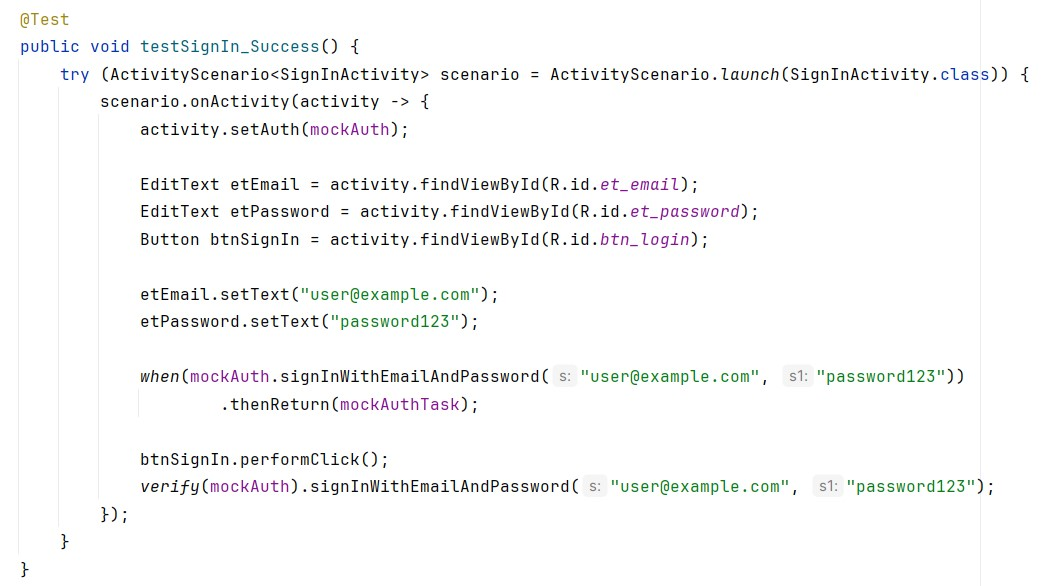
\includegraphics[width=0.8\linewidth]{img/test/test-login.jpg}}
\end{minipage}
\\


Zgodnie z założeniami test przebiegł pomyślnie, a więc funkcja działa poprawnie i pozwala użytkownikom na logowanie do aplikacji za pomocą ich danych. Poprawny przebieg testu potwierdza rys. \ref{result:login}. \\
\setlength{\fboxrule}{0.5pt}
\begin{figure}[H]
    \centering
    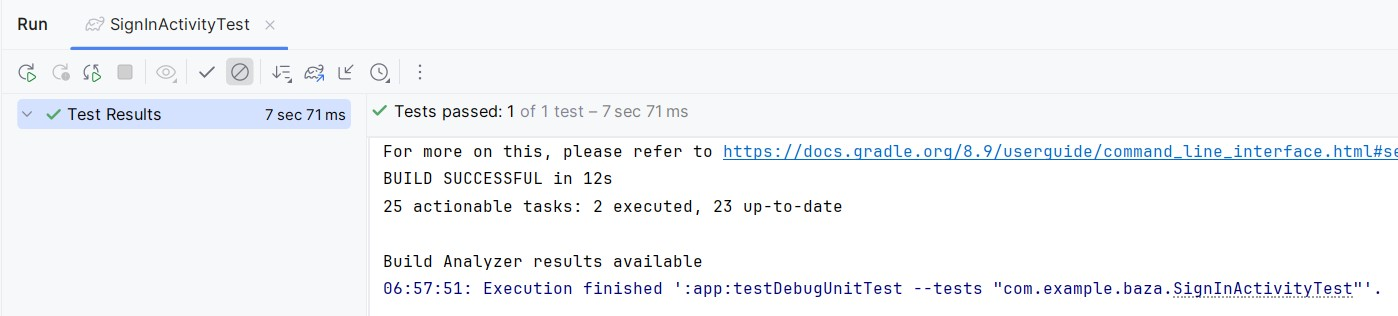
\includegraphics[scale=0.5]{img/test/login-wynik.jpg}
    \caption{Wynik testu jednostkowego sprawdzającego poprawność logowania.}
    \label{result:login}
\end{figure}

\subsection*{Test jednostkowy - rejestracja użytkownika}
Test ma na celu sprawdzenie poprawności działania funkcji rejestracji nowego użytkownika w systemie. Do tego przygotowano próbną instancję Firebase Authentication oraz przykładowego użytkownika o danych logowania: test@example.com o nazwie użytkownika TestUser z hasłem password123. Taki użytkownik nie istnieje w prawdziwej bazie danych systemu, został stworzony w klasie testowej na potrzeby  przeprowadzenia tego testu. Treść testu sprawdzającego poprawność rejestracji przedstawiona jest na listingu \ref{test:signup}. \\
\indent Zgodnie z założeniami test przebiegł pomyślnie, a więc funkcja działa poprawnie i pozwala użytkownikom na zakładanie konta w aplikacji i zapis ich danych. Poprawny przebieg testu potwierdza rys. \ref{result:login}. \\

\setlength{\fboxrule}{0.5pt}
\begin{figure}[H]
    \centering
    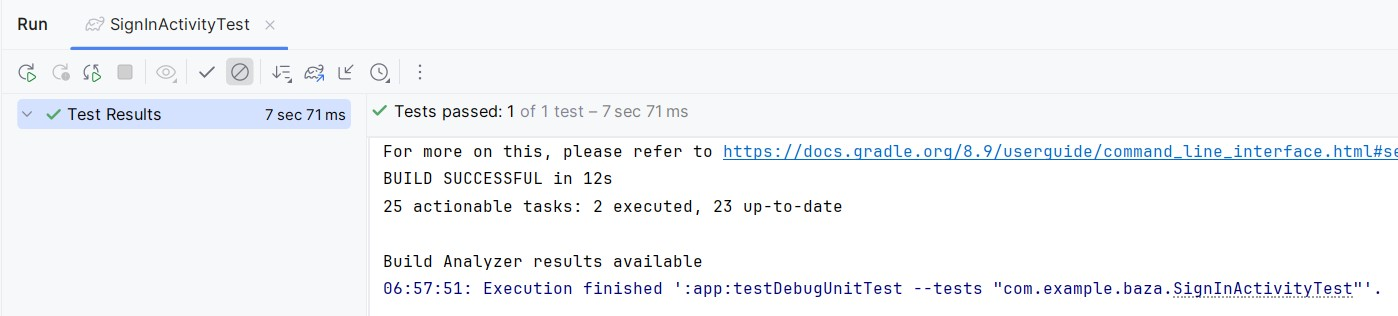
\includegraphics[scale=0.5]{img/test/login-wynik.jpg}
    \caption{Wynik testu jednostkowego sprawdzającego poprawność rejestracji nowego użytkownika.}
    \label{result:login}
\end{figure}


\noindent
\begin{minipage}{\linewidth}
    \captionof{listing}{Test jednostkowy - rejestracja.}
    \label{test:signup}
    \centering
    \fbox{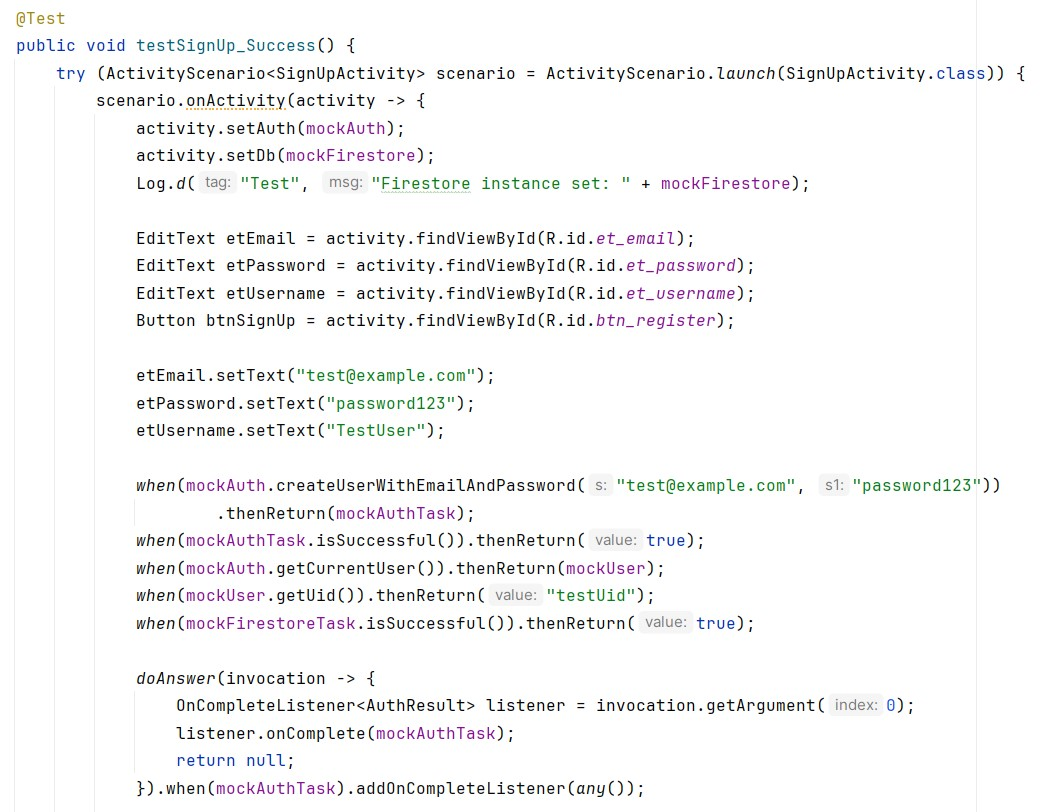
\includegraphics[width=0.8\linewidth]{img/test/test-signup1.jpg}}\\[1em]
    \fbox{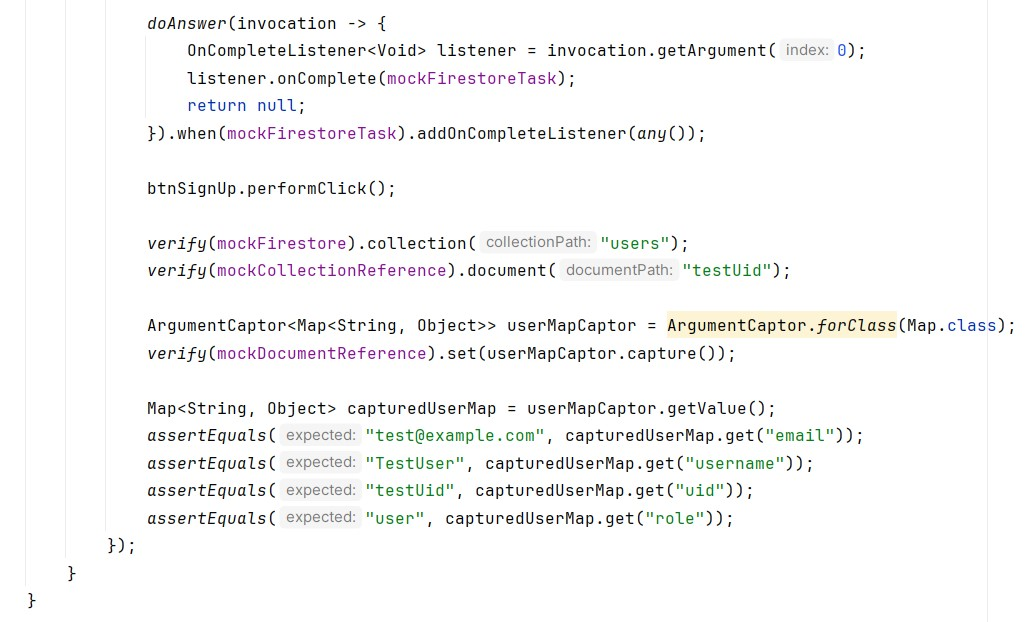
\includegraphics[width=0.8\linewidth]{img/test/test-signup2.jpg}}
\end{minipage}
\\




\subsection*{Test jednostkowy - generowanie URL trasy}
Test ma na celu sprawdzenie poprawności generowania URL z~trasą o podanym jej początku i końcu. Sprawdzono to za pomocą asercji.\\
\noindent
\begin{minipage}{\linewidth}
    \captionof{listing}{Test jednostkowy - generowanie URL.}
    \label{test:map}
    \centering
    \fbox{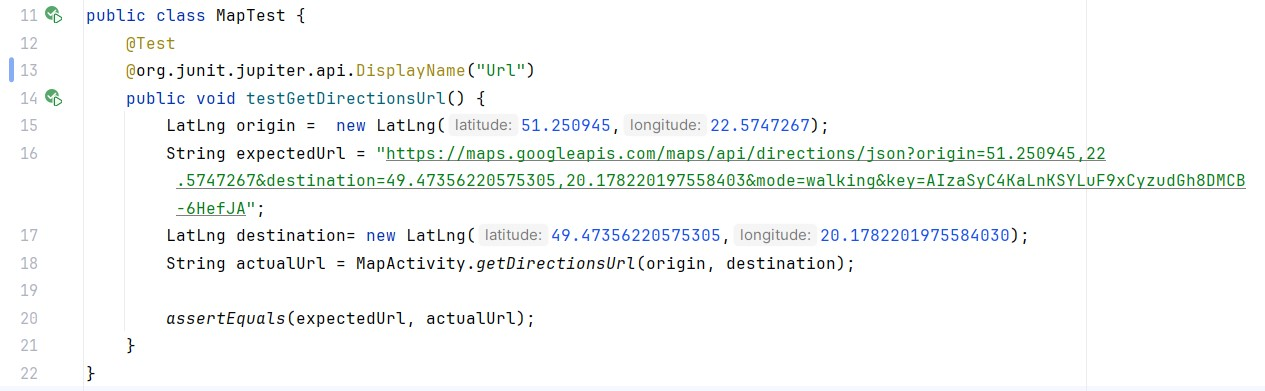
\includegraphics[width=0.8\linewidth]{img/test/testmap.jpg}}
\end{minipage}
\\
Zgodnie z założeniami test przebiegł pomyślnie, a więc funkcja działa poprawnie i generuje poprawne linki do wyznaczonej trasy na bazie jej punktu początkowego i końcowego. Poprawny przebieg testu potwierdza rys. \ref{result:map}. \\

\setlength{\fboxrule}{0.5pt}
\begin{figure}[H]
    \centering
    \fbox{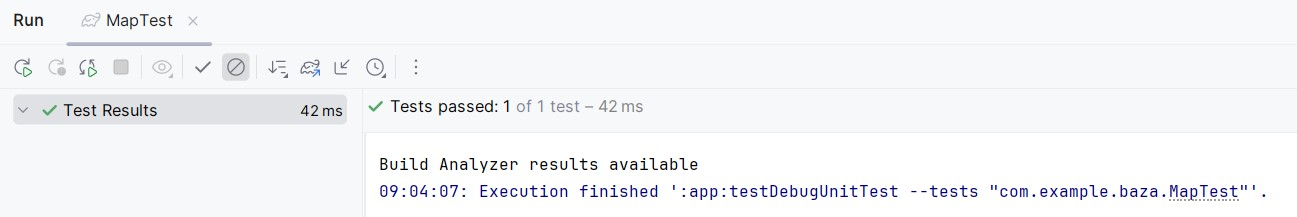
\includegraphics[scale=0.5]{img/test/maptest_wynik.jpg}}
    \caption{Wynik testu jednostkowego sprawdzającego poprawność generowania URL z~trasą o~podanym punkcie początkowym i końcowym.}
    \label{result:map}
\end{figure}

Powyższe testy przebiegły pomyślnie, funkcje zwróciły oczekiwane wartości i spełniły nasze wymagania.

\subsection{Testy manualne}
Testy manualne są ręcznym sposobem na sprawdzenie zachowania aplikacji. Tester sprawdza wtedy wszystkie możliwe dla użytkownika opcje i kombinacje kroków, które klient może wykonać choćby przez przypadek. Stosowanie testów manualnych pozwala na wykrycie luk w kodzie i funkcjonalnościach, których programista mógł nie przewidzieć lub przeoczyć. Niewykrycie niektórych niedopatrzeń może nieść za sobą fatalne skutki, jak na przykład usunięcie całej bazy danych systemu informatycznego, jeśli programista nie zabezpieczy wystarczająco dostępu do treści nieupoważnionym użytkownikom.\par
W naszej aplikacji głównymi funkcjonalnościami jest możliwość wyznaczenia trasy na mapie oraz zgłaszanie zagrożeń występujących na trasie.
\subsection*{Test manualny - wyznaczanie trasy}
Główną funkcjonalnością opisywanej aplikacji są mapy i usługi z nimi związane. Najważniejszą dostępną opcją jest wyznaczanie trasy z jednego punktu do drugiego i rysowanie jej na mapie tak, aby użytkownik widział dokładnie, gdzie się znajduje. Dlatego niniejszy test sprawdzi poprawność wykonywania tej funkcji według poniższego scenariusza:
\begin{enumerate}
    \item Przejdź do ekranu z mapą (rys. \ref{test:map1}).
    \item Wybierz funkcję wyznaczania trasy (rys. \ref{test:map2}).
    \item Wybierz punkt początkowy trasy (rys. \ref{test:map3}).
    \item Wybierz punkt końcowy trasy.
    \item Zatwierdź wybór (rys. \ref{test:map4}).
    \item Przeprowadź nawigację w aplikacji Google Maps lub idź po trasie wyświetlonej w~aplikacji (rys. \ref{test:map5}).
\end{enumerate}

\setlength{\fboxrule}{0.5pt}
\begin{figure}[H]
    \centering
    \fbox{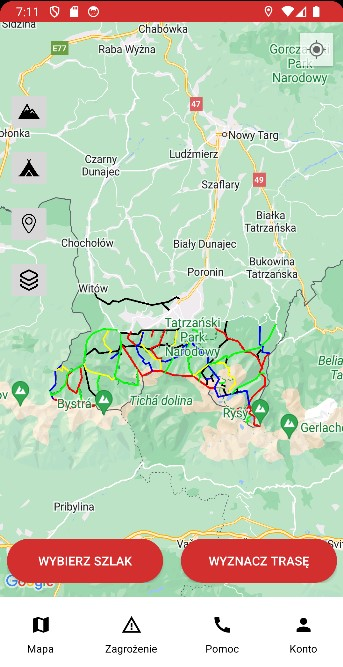
\includegraphics[scale=0.6]{img/test/testmap1.jpg}}
    \caption{Widok początkowy map.}
    \label{test:map1}
\end{figure}

Aby przejść do trybu wyznaczania trasy należy kliknąć przycisk "Wyznacz trasę" widoczny na dole ekranu na rys. \ref{test:map1}.

\setlength{\fboxrule}{0.5pt}
\begin{figure}[H]
    \centering
    \fbox{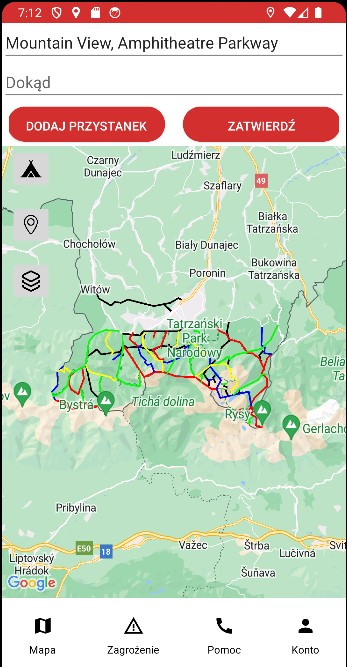
\includegraphics[scale=0.6]{img/test/testmap2.jpg}}
    \caption{Wybranie funkcji wyznaczania trasy.}
    \label{test:map2}
\end{figure}

Tryb wyznaczania trasy posiada pola wyświetlające początek i koniec trasy (rys.\ref{test:map2}), które ustawia się za pomocą markera wyświetlanego na mapie, co jest widoczne na rys. \ref{test:map3}. Ponadto jest opcja dodania przystanku, która wyznacza trasę z uwzględnieniem wybranego punktu na mapie. Na potrzeby testów ten krok został pominięty.

\setlength{\fboxrule}{0.5pt}
\begin{figure}[H]
    \centering
    \fbox{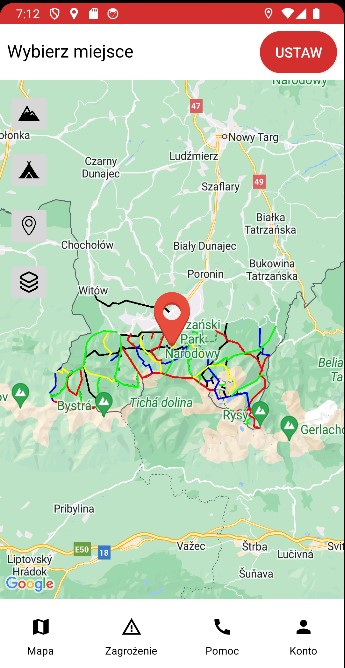
\includegraphics[scale=0.6]{img/test/testmap3.jpg}}
    \caption{Wybieranie punktu początkowego i końcowego trasy za pomocą markera.}
    \label{test:map3}
\end{figure}
\newpage
Na rys. \ref{test:map4} ukazane są markery początkowe i końcowe wybranej przez użytkownika trasy oraz słowne określenie ich położenia w górnej części ekranu. Aby trasa została wyznaczona, użytkownik musi potwierdzić swój wybór klikając "Zatwierdź". Aplikacja wtedy wyznacza trasę i rysuje ją na mapie.

\setlength{\fboxrule}{0.5pt}
\begin{figure}[H]
    \centering
    \fbox{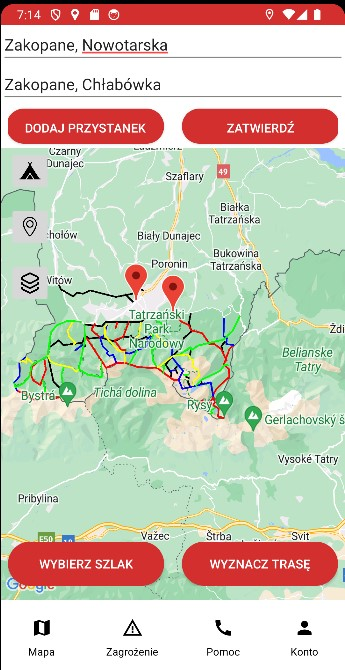
\includegraphics[scale=0.6]{img/test/testmap4.jpg}}
    \caption{Widoczne markery na początku i końcu trasy.}
    \label{test:map4}
\end{figure}

Po zatwierdzeniu wybranej trasy jest ona rysowana na mapie z pomocą koloru różowego, aby była łatwa do odróżnienia od szlaków rysowanych na mapie. Aplikacja od razu nakierowuje kamerę na początek trasy (rys. \ref{test:map5}) i jest gotowa do pokazywania użytkownikowi jego lokalizacji względem wyznaczonej trasy.

\setlength{\fboxrule}{0.5pt}
\begin{figure}[H]
    \centering
    \fbox{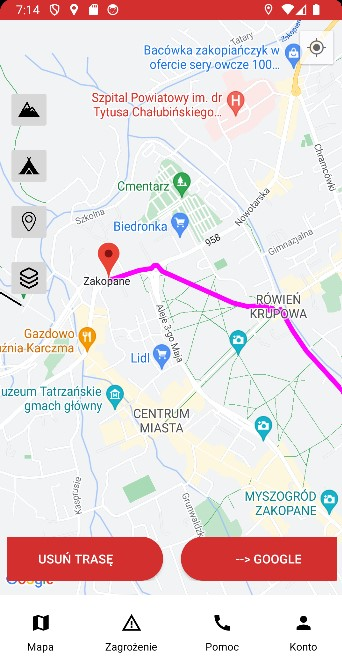
\includegraphics[scale=0.6]{img/test/testmap5.jpg}}
    \caption{Wyznaczona trasa i ukazany jej początek.}
    \label{test:map5}
\end{figure}

Przedstawoiny powyżej test przebiegł pomyślnie i potwierdził poprawne działanie funkcjonalności pozwalającej na wyznaczenie trasy z wybranego punktu początkowego do punktu końcowego. Użytkownik w tym momencie może wybrać, czy woli kierować się trasą pokazaną na mapie w aplikacji, czy woli nawigację w aplikacji Google Maps po wyznaczonej trasie.


\subsection*{Test manualny - wysyłanie zagrożeń}
Projektując aplikację miano na uwadze omylność ludzką, dlatego starano się zabezpieczyć system na różnego rodzaju błędy ludzkie i niedopatrzenia. Poniższy test sprawdzi, czy na pewno wszystkie możliwe opcje błędów zostały uwzględnione i zabezpieczone. Test manualny zostanie przeprowadzony według poniższego scenariusza.
\begin{enumerate}
    \item Przejdź do ekranu z formularzem zgłoszeń (rys. \ref{test:zglos1}).
    \item Wybierz typ zagrożenia.
    \item Podaj opis zagrożenia.
    \begin{enumerate}
        \item Nie podano opisu zagrożenia (rys. \ref{test:zglos2}).
    \end{enumerate}
    \item Naciśnij “Dodaj zagrożenie”.
    \begin{enumerate}
        \item Internet nie został włączony (rys. \ref{test:zglos3}).
        \item Lokalizacja nie została włączona (rys. \ref{test:zglos4}).
    \end{enumerate}
\end{enumerate}

\setlength{\fboxrule}{0.5pt}
\begin{figure}[H]
    \centering
    \fbox{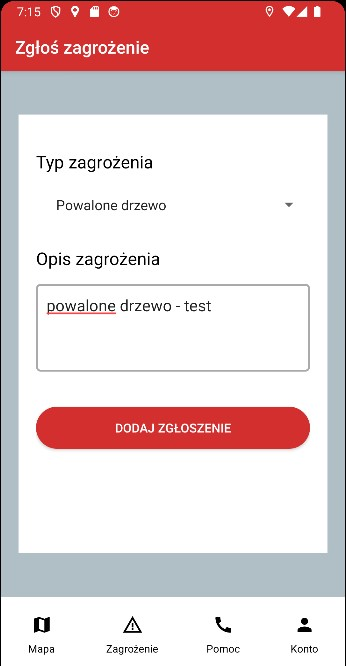
\includegraphics[scale=0.6]{img/test/testzglos1.jpg}}
    \caption{Formularz zgłaszania zagrożenia na trasie.}
    \label{test:zglos1}
\end{figure}

Formularz przedstawiony na rys. \ref{test:zglos1} wymaga od użytkownika podania typu oraz opisu zagrożenia występującego na szlaku. W przypadku braku opisu, na ekranie pojawia się komunikat, widoczny na rys. \ref{test:zglos2}, informormujący o konieczności jego uzupełnienia.
\setlength{\fboxrule}{0.5pt}
\begin{figure}[H]
    \centering
    \fbox{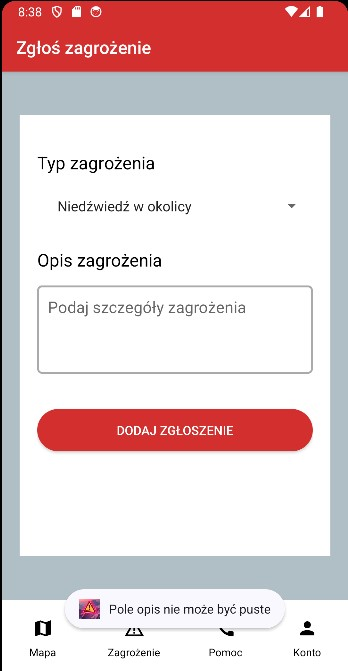
\includegraphics[scale=0.6]{img/test/testzglosopis.jpg}}
    \caption{Komunikat informujący o braku opisu zagrożenia.}
    \label{test:zglos2}
\end{figure}

W sytuacji, gdy użytkownik chce wysłać zgłoszenie, lecz w danym momencie nie ma połączenia z internetem, aplikacja wyświetla powiadomienie o braku połączenia, tak jak na rys. \ref{test:zglos3}. 
\setlength{\fboxrule}{0.5pt}
\begin{figure}[H]
    \centering
    \fbox{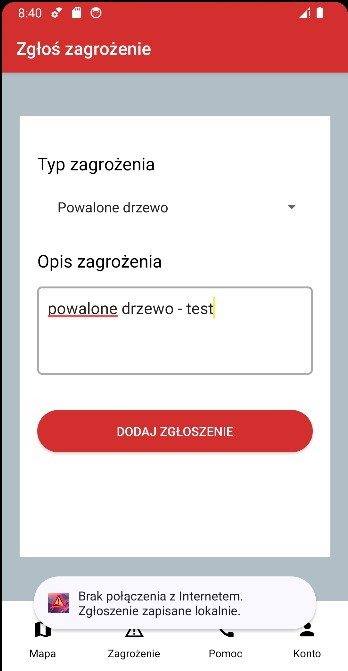
\includegraphics[scale=0.6]{img/test/brakinternetu.jpg}}
    \caption{Komunikat informujący o braku internetu.}
    \label{test:zglos3}
\end{figure}
Jednak, aby zgłoszenie zostało wysłane, użytkownik musi mieć jeszcze włączoną lokalizację, o czym informuje komunikat przedstawiony na rys. \ref{test:zglos4}. 

\setlength{\fboxrule}{0.5pt}
\begin{figure}[H]
    \centering
    \fbox{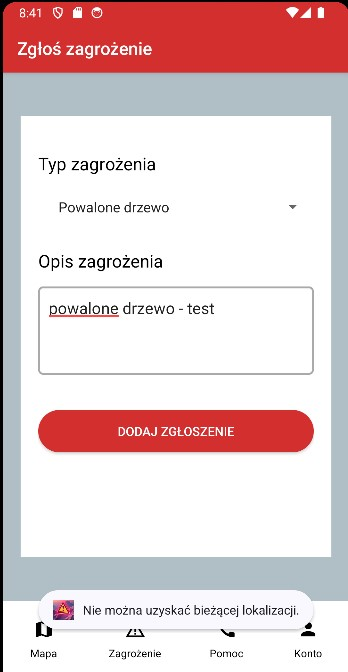
\includegraphics[scale=0.6]{img/test/braklok.jpg}}
    \caption{Komunikat informujący o braku lokalizacji.}
    \label{test:zglos4}
\end{figure}

Po kliknięciu “Zgłoś zagrożenie” i spełnieniu wszystkich wymagań, formularz zostanie pomyślnie wysłany i wyświetlony na liście zgłoszeń do zaakceptowania w interfejsie administratora (rys. \ref{test:zglos5}) . 

\setlength{\fboxrule}{0.5pt}
\begin{figure}[H]
    \centering
    \fbox{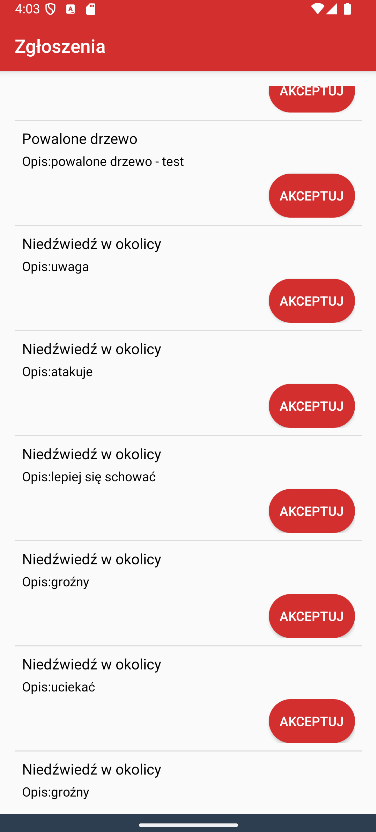
\includegraphics[scale=0.6]{img/test/testdanger.png}}
    \caption{Pomyślnie wysłane zgłoszenie i wyswietlenie go w interfejsie administratora.}
    \label{test:zglos5}
\end{figure}
Opisany test dowiódł, iż zgłoszenie zostanie wysłane tylko wtedy, gdy użytkownik poda wszystkie wymagane informacje dotyczące zagrożenia oraz będzie miał włączony internet, a~także udostępnioną lokalizację.
